% Preamble
%\documentclass[xetex,mathserif,serif]{beamer}
\documentclass{beamer}

% Packages
\usepackage[spanish]{babel}
\selectlanguage{spanish}
\usepackage[utf8]{inputenc} % For spanish (and international) letters like acents.
\usepackage{hyperref} % To create hyperlinks within the document.
\usepackage{graphicx} % To include graphics (pictures, images)
\usepackage{float} % For the use of the parameter "H" in command "\begin{figure}[H]" (i.e. exact position of image in text)
\usepackage{verbatim} % For long comments
\usepackage{tikz} % For include Dia diagrams in .tex format

\graphicspath{{../Diagramas/}} % Path of the folder containing the images

\title{Colección Archivística del LAIS}
\subtitle{Sistema de apoyo a la catalogación de archivos audiovisuales}
\author{Rodrigo Colín Rivera, Sergio Amaro Rosas}
\institute
{
  Laboratorio Audiovisual de Investigación Social\\
  Instituto de Investigaciones Dr. José María Luis Mora
}
\date{\today}
\subject{Catalogación de Acervo Documental en Video}

\begin{comment}
\AtBeginSection[]
{
  \begin{frame}
    \frametitle{Tabla de contenidos}
    \tableofcontents[currentsection]
  \end{frame}
}
\AtBeginSubsection[]
{
  \begin{frame}
    \frametitle{Tabla de contenidos}
    \tableofcontents[currentsection,currentsubsection]
  \end{frame}
}
\end{comment}

% Style and theme
\usetheme{PaloAlto}
%\usecolortheme{orchid} %crane,dolphin,lily

% Document environment
\begin{document}

\frame{\titlepage} % Página inicial

\section{Introducción}
\begin{frame}
	\frametitle{Introducción}
	El Laboratorio Audiovisual de Investigación Social (LAIS) del Instituto de Investigación Dr. José María Luis Mora se propusó abocarse en la labor de construir un \textbf{acervo} debidamente documentado, ponerlo en acceso para consulta y potenciar así la investigación con este tipo de materiales.

	El LAIS consta de una colección archivística para materiales audiovisuales cuyos registros actuales se encuentran en formato de \textbf{hojas de cálculo} que integran la ficha de documentación.
	
	Los problemas actuales consisten en que es \textbf{complicado buscar} o filtrar los registros, la integridad de la información, el control de acceso y la manipulación de los datos.
\end{frame}

\section{Propuesta}
\begin{frame}
	\frametitle{Propuesta}
	\framesubtitle{Creación de un sistema computacional para la catalogación de archivos audiovisuales}
	
	La propuesta consiste en crear una \textbf{base de datos} para el manejo actual y futuro de las fichas de documentación de los materiales audiovisuales del LAIS junto con una \textbf{interfaz de usuario} que permita manipular fácilmente la base de datos.
\end{frame}

\section{Esquema general}
\begin{frame}
	\frametitle{Esquema general del sistema}
	\begin{figure}[H]
		\centering
		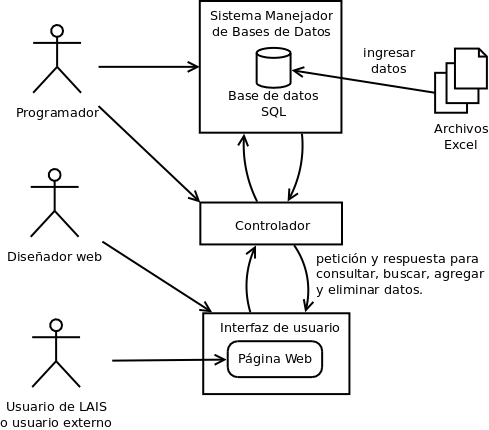
\includegraphics[width=0.7\textwidth]{EsquemaGeneral.png}
		\caption{Esquema general del sistema de consulta}
		\label{fig:esquema_general}
	\end{figure}
\end{frame}

\section{Casos de uso}
\begin{frame}
	\frametitle{Diagrama de casos de uso}
	\begin{figure}[H]
		\centering
		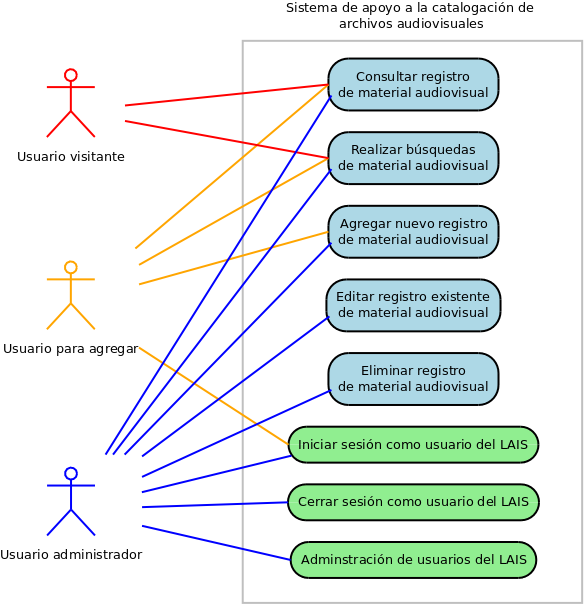
\includegraphics[width=0.6\textwidth]{CasosDeUso.png}
		\caption{Diagrama de casos de uso}
		\label{fig:caso_de_uso}
	\end{figure}
\end{frame}

\section{Acerca del desarrollo de software}
\begin{frame}
	\frametitle{Desarrollo de software}
	\framesubtitle{Consideraciones}
	Para el tipo de sistema que se desea desarrollar es recomendable tomar en cuenta los siguientes aspectos:
	\begin{itemize}
		\item Arquitectura Modelo-Vista-Controlador
		\item Sistema Manejador de Contenido
		\item Documentación asociada e ingeniería de software
	\end{itemize}
\end{frame}

\section{Kanban}
\begin{frame}
	\frametitle{Tareas desarrolladas}
	\begin{itemize}
		\item Diseño de la base
		\item Vistas de las páginas
		\item Funcionalidad para realizar búsqueda
		\item Autentificación y administración de usuarios
		\item Administración de archivos audiovisuales
		\item Mostrar contenido de audiovisuales
		\item Migrar la base de datos
		\item Configurar servidor
	\end{itemize}
\end{frame}

\section{Diagrama de navegación}
\begin{frame}
	\frametitle{Diagrama de navegación}
	\framesubtitle{\href{http://localhost/lais-audiovisual/public/}{LAIS Audiovisual}}	
	\begin{figure}[H]
		\centering
		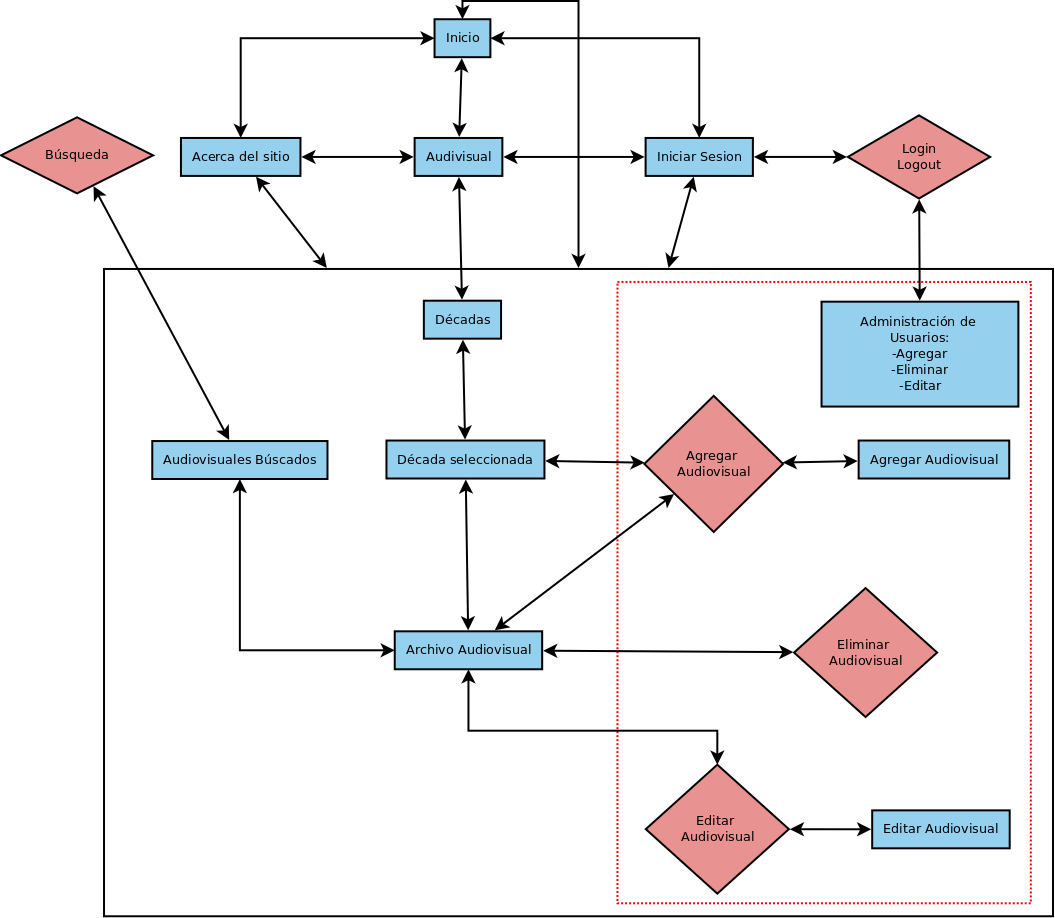
\includegraphics[width=0.7\textwidth]{navegacion.png} % CAMBIAR IMAGEN
		\caption{Mapa de navegación de LAIS Audiovisual}
		\label{fig:esquema_general}
	\end{figure}
\end{frame}

\section{Conclusión}
\begin{frame}
	\frametitle{Conclusiones}
	\begin{itemize}
		\item Se logró implementar satisfactoriamente la parte principal del sistema que cumple con la arquitectura MVC y permite la administración completa de archivos audiovisuales y usuarios.
		\item Durante el desarrollo, siempre tener como objetivo la creación de un sistema capaz de organizarse y administrarse de manera simple por parte de los usuarios del LAIS sin la necesidad de intervención de los programadores.
		\item Crear y mantener una base de datos estandarizada para reutilizar esa información mediante un manejo semántico de contenido (siguiente proyecto a desarrollar).
	\end{itemize}
\end{frame}

\begin{frame}
	\begin{center}
		GRACIAS POR SU TIEMPO.
		
		
\includegraphics{scientistapprovedfutura.png}
	\end{center}
\end{frame}

\end{document}